\documentclass[12pt]{article}
\usepackage[pdftex]{graphicx}
\usepackage{amsfonts}
\usepackage[italian]{babel}
\usepackage{graphicx}
\usepackage{color}
\usepackage{multirow,bigdelim}
\usepackage{relsize}
\usepackage{fdsymbol}
\usepackage{mdframed}

\definecolor{grey}{rgb}{0.3,0.3,0.3}
\definecolor{verylightgray}{rgb}{.97,.97,.97}
\definecolor{lightred}{rgb}{1,.70,.70}

\usepackage{listings, framed}
\lstset{
  language=Java,
  showstringspaces=false,
  columns=flexible,
  basicstyle={\small\ttfamily},
  frame=none,
  numbers=none,
  keywordstyle=\bfseries\color{grey},
  commentstyle=\itshape\color{red},
  identifierstyle=\color{black},
  stringstyle=\color{blue},
  numberstyle={\ttfamily},
%  breaklines=true,
  breakatwhitespace=true,
  tabsize=3,
  escapechar=|
}

\mdfsetup{font=\scriptsize}

\def\codesize{\smaller}
\def\<#1>{\codeid{#1}}
\newcommand{\codeid}[1]{\ifmmode{\mbox{\codesize\ttfamily{#1}}}\else{\codesize\ttfamily #1}\fi}

%****************enlarge layout
\textheight     243.5mm
\topmargin      -20.0mm
\textwidth      500pt
\hoffset        -80pt
%*****************theorems and such
\newcounter{esnu}
\newenvironment{esercizio}{\medskip \noindent {\bf Esercizio\addtocounter{esnu}{1} \arabic{esnu}}}{}
\pagestyle{empty}
\newcommand{\liff}{\mathrel{\leftrightarrow}}   % Logical IFF Symbol
\newcommand{\metaiff}{\Longleftrightarrow}      %iff in metatheory

\begin{document}

\begin{center}
  \textbf{Esame di Programmazione II, 1 febbraio 2024}\\
  (si consegnino \texttt{Sudoku.java}, \texttt{Main.java} ed eventuali classi ausiliarie che avete scritto)
\end{center}

\emph{
Si crei un progetto Eclipse e
il package \<it.univr.sudoku>. Si copino al suo interno
le classi del compito.
Non si modifichino le dichiarazioni dei metodi e delle classi. Si possono definire altri campi,
metodi o costruttori, ma devono essere \<private>. Si possono definire altre classi,
che in tal caso vanno consegnate.
La soluzione che verr\`a consegnata dovr\`a compilare,
altrimenti non verr\`a corretta.}

\vspace*{2ex}

Un sudoku \`e un gioco consistente in una griglia 9x9, divisa internamente in nove
regioni 3x3, in cui sono posizionati dei numeri da 1 a 9. Alcune caselle
possono essere lasciate vuote. Per esempio, questo \`e un sudoku:
%
\begin{center}
  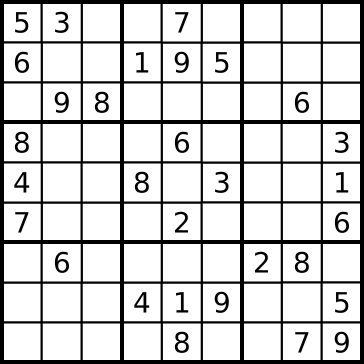
\includegraphics[width=0.25\textwidth]{sudoku}
\end{center}
%
Si richiede inoltre che i numeri in un sudoku siano
unici all'interno di ciascuna riga, di ciascuna colonna e di ciascuna regione.
Si noti che, tradizionalmente, i sudoku contengono numeri da 1 a 9, ma nessuno
impedisce l'esistenza di sudoku in cui le nove alternative vengano rappresentate
con nove oggetti di un tipo generico \<E>. Per questo, la classe di partenza di questo compito
\`e generica: \<Sudoku$\langle$E$\rangle$>. Tale classe possiede un costruttore
che genera un sudoku casuale e che riceve:
\begin{enumerate}
\item il numero \<empty> di caselle che devono essere lasciate vuote
  nel sudoku;
\item una funzione che indica come rappresentare le nove alternative con
  un oggetto di classe \<E>. Tale funzione \`e data come un'implementazione
  dell'interfaccia di libreria \<IntFunction$\langle$E$\rangle$>:
  ha solo un metodo che dato un intero tra 1 e 9 restituisce un oggetto
  di tipo \<E> che indica come rappresentare tale numero nel sudoku.
\end{enumerate}
%
Per esempio, un sudoku tradizionale avrebbe tipo \<Sudoku$\langle$Integer$\rangle$>
e il suo costruttore riceve una funzione che mappa 1 in \<Integer.valueOf(1)>,
2 in \<Integer.valueOf(2)>, \ldots, 9 in \<Integer.valueOf(9)>.

\vspace*{2ex}\textbf{Esercizio 1 ($2$ punti).}
Si completi il costruttore di \<Sudoku> in modo da lanciare un'eccezione
di tipo \<IllegalArgumentException> se \<empty> non fosse tra 0 e 61 inclusi.

\vspace*{2ex}\textbf{Esercizio 2 ($7$ punti).}
Si completino i metodi \<isHorizontallyUnique>, \<isVerticallyUnique> e
\<isUniqueInRegion> di \<Sudoku>, che determinano se un elemento
del sudoku \`e unico nella sua riga, nella sua colonna e nella sua
regione, rispettivamente.

\vspace*{2ex}\textbf{Esercizio 3 ($7$ punti).}
Si completi il metodo \<hide> di \<Sudoku>, che rende vuote esattamente
\<howMany> caselle a caso del sudoku che non siano gi\`a vuote.
Si noti che, nella matrice con cui \`e implementato il sudoku,
le caselle vuote vengono rappresentate con il numero 0.

\vspace*{2ex}\textbf{Esercizio 4 ($7$ punti).}
Si completi il metodo \<toString> di \<Sudoku>,
che restituisce una stringa che descrive il sudoku, come quelle che
vedete nelle stampe che seguono.
\textbf{Suggerimento:} potrebbe esservi utile il metodo
\<repeat> delle stringhe, che restituisce una stringa ripetuta
pi\`u volte.

\vspace*{2ex}\textbf{Esercizio 5 ($8$ punti).}
Si completi la classe \<Main> in modo da creare i cinque sudoku indicati
nel suo codice prima delle loro cinque stampe.

\vspace*{2ex}
\hrule
\vspace*{2ex}

Se tutto \`e corretto, l'esecuzione del \texttt{Main} stamper\`a
qualcosa del tipo:

\begin{center}
  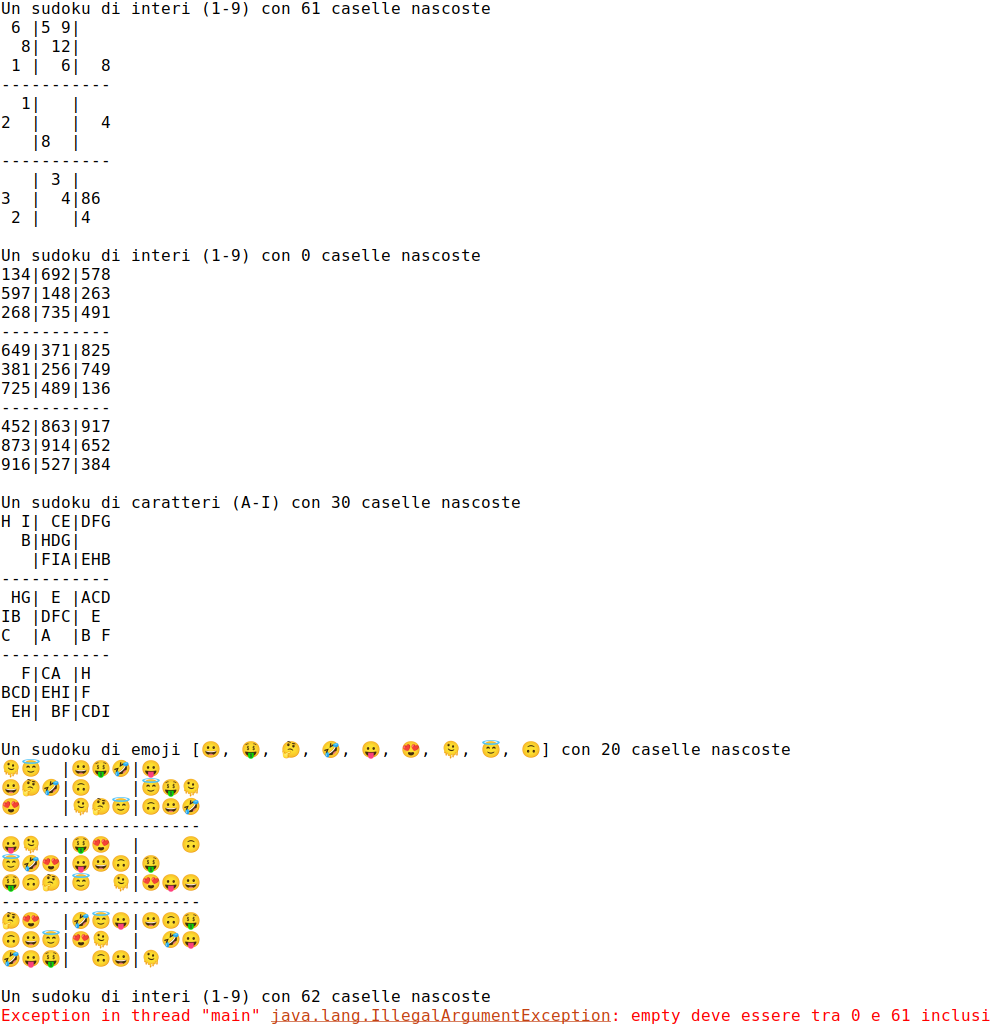
\includegraphics[width=\textwidth]{print}
\end{center}

\end{document}
